\chapter{\label{chap:intro}Análise e Discussão}
 




\section{Resultados da \textit{Survey}}

Após a conclusão do processo de coleta dados, com o objetivo de entender quais são as preocupações de desenvolvedores de software móveis no desenvolvimento de aplicações, destaca-se nessa seção o resultado obtido na survey. A survey teve um total de 20 respondentes.

O público que respondeu essa pesquisa tem em média 5 anos de experiência com desenvolvimento de aplicações  para dispositivos móveis. Em sua maioria tem experiência com a plataforma Android e desenvolve aplicativos de uso empresarial com desenvolvimento realizado em equipe.
%falar das oturas pçataformas e dos aplicativos desenvolvidos

A norma ISO 27002 na sua seção 9 aborda boas práticas de controle de acesso que tem como objetivo como objetivos limitar o acesso à informação e aos recursos de processamento da informação, assegurar acesso de usuário autorizado e prevenir acesso não autorizado a sistemas, serviços e aplicações. Percebe-se pelas respostas desta \textit{survey}, que a maioria dos itens da seção já se tornaram práticas adotadas pelos desenvolvedores mobile. Por outro lado algumas questões como a 2.2, 2.8, 2.9, 2.10, 2.11, 2.12 não tiveram uma unanimidade muito forte nas suas respostas, o que pode indicar a falta de entendimento sobre o assunto ou falta de preocupação. 

A norma ISO 27002 na sua seção 10 aborda boas práticas de criptografia que tem como objetivo assegurar o uso efetivo e adequado da criptografia para proteger a confidencialidade, autenticidade e a integridade da informação. A única questão que não demonstrou uma unanimidade forte foi a 3.2, possivelmente pelo não entendimento da questão

A norma ISO 27002 na sua seção 12 aborda boas praticas para garantir a segurança das operações que tem como objetivo garantir a operação segura e correta dos recursos de processamento da informação, assegurar que as informações e os recursos de processamento da informação estão protegidos contra \textit{malware}, a proteção contra perda de dados, registrar eventos e gerar evidências, assegurar a integridade dos sistemas operacionais e prevenir a exploração de vulnerabilidades técnicas e minimizar o impacto das atividades de auditoria nos sistemas operacionais. Percebe-se pelas respostas desta \textit{survey}, que a maioria dos itens da seção já se tornaram práticas adotadas pelos desenvolvedores mobile.  Por outro lado as questões 5.3, 5.4 e 5.5 não tiveram uma unanimidade forte.


A norma ISO 27002 na sua seção 14 aborda boas praticas para garantir a aquisição, desenvolvimento e manutenção de sistemas com o objetivo de garantir que a segurança da informação seja parte integrante de todo o ciclo de vida dos sistemas de informação, garantir que a segurança da informação esteja projetada e implementada no ciclo de vida de desenvolvimento dos sistemas de informação e assegure a proteção dos dados usados para teste. Percebe-se pelas respostas desta \textit{survey}, que a maioria dos itens da seção já se tornaram práticas adotadas pelos desenvolvedores mobile. Por outro lado percebe-se que algumas questões como a 6.6, 6.7, 6.11 e 6.14 não tiveram uma unanimidade muito forte nas suas respostas, o que pode indicar a falta de entendimento sobre o assunto ou falta de preocupação.

\todo[inline]{A ideia seria que cada um desses parágrafos fosse no final de cada controle porém não estou conseguindo coloca-los na ordem certa como eu formato corretamente?}

 



\begin{figure}[!b]
\centering
\paragraph{
Os respondentes foram questionados sobre sua preocupação com o controle de acesso de usuários nos sistemas que desenvolvem. Os resultados são apresentados na figura \ref{fig:1.1}
}
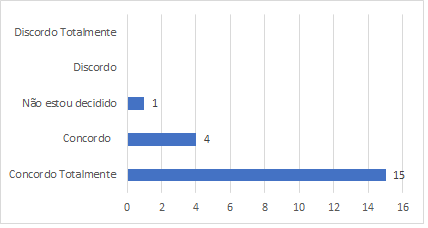
\includegraphics[scale=0.8]{figuras das questoes/1.1.PNG}
\caption{Respostas questão 1.1}

\paragraph{
Noventa e cinco por cento (95{\%}) dos respondentes (\ref{fig:1.1}) concordam que o controle de acesso em sistemas desenvolvidos é importante, considerando tanto aqueles que concordam totalmente (85{\%}) quanto aqueles que consideram a questão importante (10{\%}). Com esse resultado fica claro que existe uma preocupação dos desenvolvedores mobile com o controle de acesso de usuários.
}

\label{fig:1.1}
\end{figure}
%aqui acaba um figura
%--------------------------%
%aqui começa uma figura
\begin{figure}[!t]
\centering
\paragraph{Os respondentes foram questionados sobre sua preocupação em criar ou utilizar funcionalidades que permitam a remoção ou bloqueio de usuários no sistema. Os resultados são apresentados na figura \ref{fig:1.2}.}
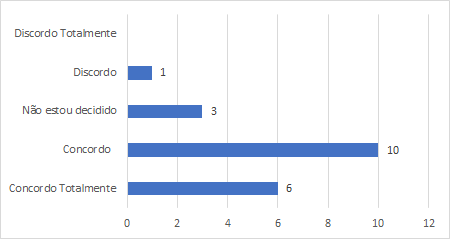
\includegraphics[scale=0.8]{figuras das questoes/1.2.PNG}
\caption{Respostas questão 1.2}

\paragraph{
Oitenta por cento (80{\%}) dos respondentes \ref{fig:1.2} concordam que criar funcionalidades que permitam remoção, bloqueio, ou desabilitação de usuários é importante, considerando tanto aqueles que concordam totalmente (30{\%}) quanto aqueles que consideram a questão apenas importante (50{\%}). Com o resultado fica claro que existe uma preocupação dos desenvolvedores com a criação destas funcionalidades.
}
\label{fig:1.2}
\end{figure}
%aqui acaba um figura
%--------------------------%
%aqui começa uma figura
\begin{figure}[!t]
\centering

\paragraph{
Os respondentes foram questionados sobre sua preocupação em desenvolver funções que permitem alteração de permissão no sistema para todos os usuários, para que seja possível fazer um gerenciamento de usuários. Os resultados são apresentados na figura \ref{fig:1.3}.
}
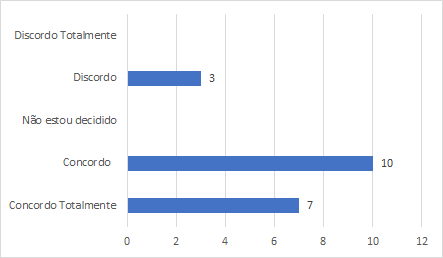
\includegraphics[scale=0.7]{figuras das questoes/1.3.png}
\caption{Respostas questão 1.3}

\paragraph{ 
Oitenta e cinco por cento (85{\%}) dos participantes afirmam se preocupar em desenvolver funcionalidades para a alteração de permissão de usuários no sistema, considerando tanto aqueles que concordam totalmente (35{\%}), quanto aqueles que consideram a questão apenas importante (50{\%}). Com esse resultado fica claro a preocupação dos desenvolvedores com a criação de tais funcionalidades. 
}

\label{fig:1.3}
\end{figure}
%aqui acaba uma figura
%--------------------------%
%aqui começa uma figura
\begin{figure}[!t]
\centering
\paragraph{
Os participantes foram questionados sobre a preocupação em criar um registro central de direitos de acesso para cada usuário. Os resultados podem ser vistos na figura \ref{fig:1.4}.
}
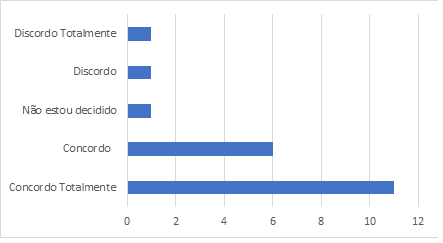
\includegraphics[scale=0.7]{figuras das questoes/1.4.png}
\caption{Respostas questão 1.4}

\paragraph{
Oitenta e cinco por cento (85{\%}) dos participantes se preocupam em criar um registro central de direitos de acesso para cada usuário, considerando tanto aqueles que concordam totalmente (55{\%}), quando aqueles que consideram apenas importante (30{\%}). Com esse resultado é possível afirmar que existe uma preocupação dos desenvolvedores com um registro central de direitos de acesso dos usuários.
}

\label{fig:1.4}
\end{figure}
%aqui acaba uma figura
%--------------------------%
%aqui começa uma figura
\begin{figure}[!t]
\centering
\paragraph{Os participantes foram questionados sobre sua preocupação em desenvolver funcionalidades que verifiquem a identidade de usuário antes de fornecer uma informação de autenticação secreta. Os resultados são apresentados na figura \ref{fig:2.1}.
}
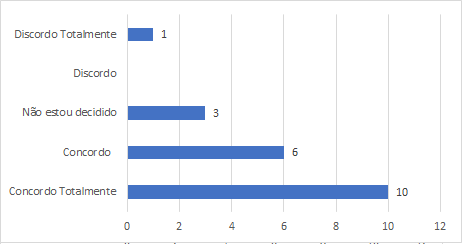
\includegraphics[scale=0.7]{figuras das questoes/2.1.png}
\caption{Respostas questão 2.1}
\paragraph{
Oitenta por cento (80{\%}) dos participantes se preocupam em desenvolver funcionalidades que verifiquem a identidade de um usuário antes de fornecer informação de autenticação secreta, considerando tanto aqueles que concordam totalmente (50{\%}) , quanto aqueles que apenas concordam (30{\%}) com a questão. Com esse resultado é possível afirmar que os desenvolvedores se preocupam com a criação de funcionalidades que verifiquem a identidade do usuário.
}
\label{fig:2.1}
\end{figure}
%aqui acaba uma figura
%--------------------------%
%aqui começa uma figura
\begin{figure}[!t]
\centering
\paragraph{Os participantes foram questionados sobre sua preocupação a respeito do aprimoramento de funcionalidades de autenticação secreta para acessos em sistemas. Os resultados podem ser consultados na figura \ref{fig:2.2}.}
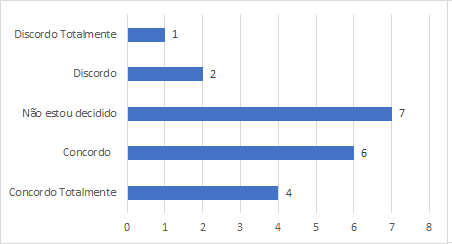
\includegraphics[scale=0.7]{figuras das questoes/2.2.png}
\caption{Respostas questão 2.2}
\paragraph{Cinquenta por cento (50{\%}) dos participantes se preocupam em aprimorar funcionalidades de autenticação secreta em acessos nos sistemas que desenvolvem, entretanto 35{\%} não foi capaz de emitir uma opinião a respeito da pergunta e 15{\%} discorda de ser uma preocupação necessária. Com esse resultado não é capaz de afirmar se existe uma preocupação dos desenvolvedores pois grande parte do grupo não foi capaz de emitir uma opinião a respeito do tema}
\label{fig:2.2}
\end{figure}
%aqui acaba uma figura
%--------------------------%
%aqui começa uma figura
\begin{figure}[!t]
\centering

\paragraph{
Os participantes foram questionados sobre a preocupação de manter a informação de autenticação secreta temporária e única pra cada pessoa. Os resultados podem ser consultados na figura \ref{fig:2.3}
}

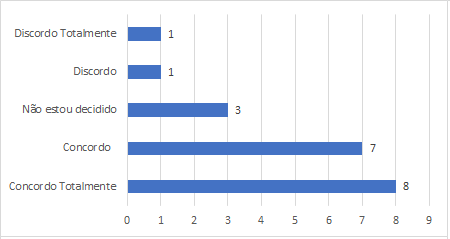
\includegraphics[scale=0.7]{figuras das questoes/2.3.png}
\caption{Respostas questão 2.3}

\paragraph{
Setenta e cinco por cento (75{\%}) dos participantes se preocupam em manter a informação de autenticação secreta única e temporária para cada pessoa, considerando tanto aqueles que concordam totalmente (40{\%}), quanto aqueles que apenas concordam (35{\%}). Com o resultado fica claro que existe uma preocupação dos desenvolvedores com o cuidado da autenticação secreta.
}

\label{fig:2.3}
\end{figure}
%aqui acaba uma figura
%--------------------------%
%aqui começa uma figura
\begin{figure}[!t]
\centering
\paragraph{
Os participantes foram questionados sobre a preocupação em fornecer recursos para que o usuário reguarde sua privacidade durante o processo de autenticação. Os resultados podem ser consultados na figura \ref{fig:2.4}
}

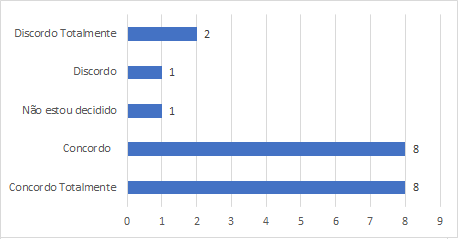
\includegraphics[scale=0.7]{figuras das questoes/2.4.png}
\caption{Respostas questão 2.4}

\paragraph{
Oitenta por cento (80{\%}) dos participantes se preocupam em fornecer recursos que possibilitem ao usuário resguardar sua privacidade durante o processo de autenticação, considerando tanto aqueles que concordam totalmente (40{\%}), quanto aqueles que apenas concordam (40{\%}). Com o resultado fica claro que existe uma preocupação dos desenvolvedores em fornecer recursos que resguardem a privacidade do usuário.
}

\label{fig:2.4}
\end{figure}
%aqui acaba uma figura
%--------------------------%
%aqui começa uma figura
\begin{figure}[!t]
\centering

\paragraph{
Os participantes foram questionados sobre a preocupação de não mostrar dados sensíveis de usuários até o processo de Log-on. Os resultados podem ser consultados na figura \ref{fig:2.5}
}

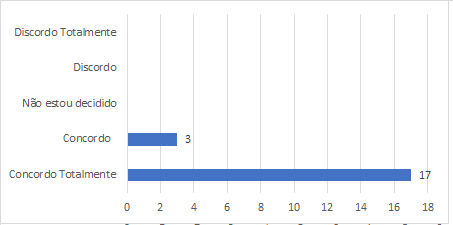
\includegraphics[scale=0.7]{figuras das questoes/2.5.png}
\caption{Respostas questão 2.5}

\paragraph{
Cem por cento (100{\%}) dos participantes se preocupam em não mostrar dados sensíveis dos usuários durante o processo de Log-on. Com o resultado é possível ver a unanimidade na importância que os desenvolvedores dão a essa questão.
}
\label{fig:2.5}
\end{figure}
%aqui acaba uma figura
%--------------------------%
%aqui começa uma figura
\begin{figure}[!t]
\centering
\paragraph{
Os participantes foram questionados sobre a preocupação de validar as informação de entrada no sistema somante quando os dados estiverem completos.Os resultados podem ser consultados na figura \ref{fig:2.6}
}
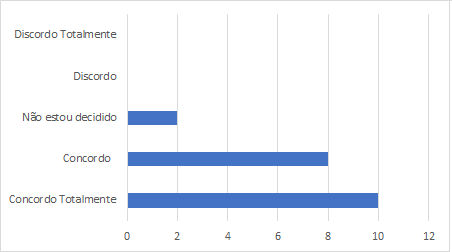
\includegraphics[scale=0.7]{figuras das questoes/2.6.png}
\caption{Respostas questão 2.6}

\paragraph{
Noventa por cento (90{\%}) dos participantes se preocupam em validar os dados de entrada no sistema somente quando estiverem completos, considerando tanto aqueles que concordam totalmente (50{\%}), quanto aqueles que apenas concordam (40{\%}). Com esse resultado fica claro que existe uma preocupação dos desenvolvedores em validar os dados do usuário somente quando estiverem totalmente completos.
}
\label{fig:2.6}
\end{figure}
%aqui acaba uma figura
%--------------------------%
%aqui começa uma figura
\begin{figure}[!t]
\centering

\paragraph{
Os participante foram questionados sobre a preocupação de não revelar qual parte do dado esta correto ou incorreto durante um processo de entrada no sistema. Os resultados podem ser consultados na figura \ref{fig:2.7}
} 

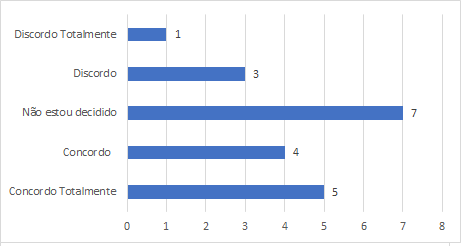
\includegraphics[scale=0.7]{figuras das questoes/2.7.png}
\caption{Respostas questão 2.7}
%\todo[inline]{trocar o gráfico ele esta errado}
\paragraph{
Oitenta e cinco por cento (85{\%}) dos participantes se preocupam em não revelar qual parte do dado esta correto ou incorreto em um processo de entrada no sistema, considerando tanto aqueles que concordam totalmente (65{\%}), quanto aqueles que apenas concordam (20{\%}). Com esse resultado fica claro a preocupação do desenvolvedores em não fornecer ajuda a um usuário possivelmente mal intencionado.
}
\label{fig:2.7}
\end{figure}
%aqui acaba uma figura
%--------------------------%
%aqui começa uma figura
\begin{figure}[!t]
\centering

\paragraph{Os participantes foram questionados sobre a preocupação de proteger o sistema contra tentativas consecutivas de entrada forçada no sistema. Os resultados podem ser consultados na figura \ref{fig:2.8}.
}

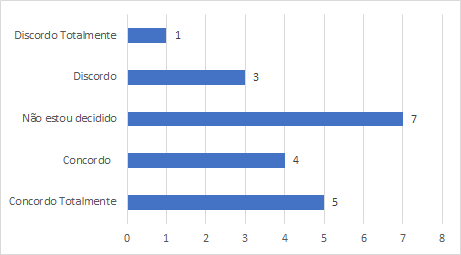
\includegraphics[scale=0.7]{figuras das questoes/2.8.png}
\caption{Respostas questão 2.8}

\paragraph{
Quarenta e cinco por cento (45{\%}) dos participantes se preocupam em proteger o sistema contra tentativas consecutiva de entrada forçada no sistema, contudo 35{\%} dos respondentes não foi capaz de opinar sobre a questão e 20{\%} discorda que seja um preocupação.Com esse resultado não é possível afirmar se existe uma preocupação dos desenvolvedores com proteção do sistema contra um tentativa forçada de entrada no sistema.
}

\label{fig:2.8}
\end{figure}
%aqui acaba uma figura
%--------------------------%
%aqui começa uma figura
\begin{figure}[!t]
\centering
\paragraph{Os participantes foram questionados sobre a preocupação de comunicar um evento de segurança caso uma tentativa ou violação bem sucedida de entrada no sistema seja realizada. Os resultados podem ser consultados na figura \ref{fig:2.9}.}
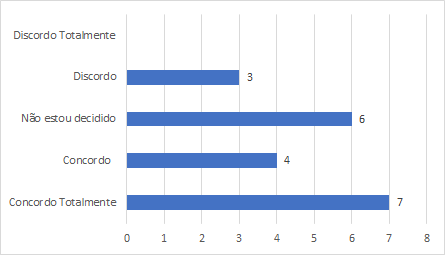
\includegraphics[scale=0.7]{figuras das questoes/2.9.png}
\caption{Respostas questão 2.9}

\paragraph{Cinquenta e cinco por cento (55{\%}) dos participantes se preocupam em comunicar eventos de segurança, contudo 30{\%} não souberam responder e 15{\%} discordaram. Com esse resultado é possível afirmar que existe uma preocupação dos desenvolvedores sobra a comunicação de eventos de segurança.} 

\label{fig:2.9}
\end{figure}
%aqui acaba uma figura
%--------------------------%
%aqui começa uma figura
\begin{figure}[!t]
\centering
\paragraph{Os participante foram questionados sobre a preocupação encerrar sessões após um período de inatividade. Os resultados podem ser consultados na figura \ref{fig:2.10}.}

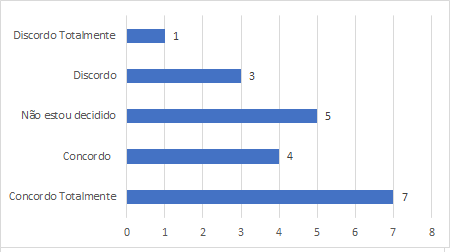
\includegraphics[scale=0.7]{figuras das questoes/2.10.png}
\caption{Respostas questão 2.10}

\paragraph{Cinquenta e cinco por cento (55{\%}) dos participantes se preocupam em encerrar sessões inativas após um período de inatividade, contudo 25{\%} não soube opinar e 20{\%} discordaram que seria uma preocupação. Com esse resultado é possível  ver que existe uma preocupação dos desenvolvedores quanto ao tempo de inatividade.
}
\label{fig:2.10}
\end{figure}

%aqui acaba uma figura
%--------------------------%
%aqui começa uma figura

\begin{figure}[!t]
\centering
\paragraph{Os participantes foram questionados sobre a preocupação em criar sistemas que obriguem a escolha de uma senha de qualidade por parte do usuário. Os resultados podem ser consultados na figura \ref{fig:2.11}. }

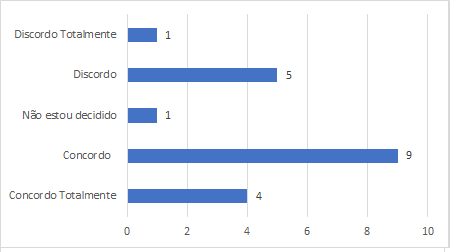
\includegraphics[scale=0.7]{figuras das questoes/2.11.png}
\caption{Respostas questão 2.11}

\paragraph{
sessenta e cinco por cento (65{\%}) dos participantes se preocupa em obrigar o usuário a criar um senha de qualidade, entretanto 30{\%} descorda que  isso seja uma preocupação. Com o resultado é possível afirmar que existe uma preocupação dos desenvolvedores em obrigar o usuário criar senhas de qualidade, \todo[inline]{entretanto seria relevante entender o motivo que levou os 30{\%} dos participantes a discordarem da importância.} 
}

\label{fig:2.11}
\end{figure}

%aqui acaba uma figura
%--------------------------%
%aqui começa uma figura

\begin{figure}[!t]
\centering
\paragraph{Os participantes foram questionados sobre a preocupação em desenvolver sistemas que obriguem o usuário a mudar as suas senhas temporárias no primeiro acesso ao sistema. Os resultados podem ser consultados na figura \ref{fig:2.12}. }
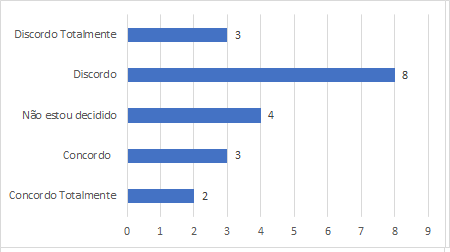
\includegraphics[scale=0.7]{figuras das questoes/2.12.png}
\caption{Respostas questão 2.12}
\paragraph{
Cinquenta e cinto por cento (55{\%}) dos respondentes dos participantes não se preocupam em obrigar o usuário a trocar a senha temporária de primeiro acesso, 20{\%} não soube responder e Apenas 25{\%} dos participantes concordaram que obrigar a troca de senha seria uma preocupação. Com esse resultado é possível concluir que não existe uma preocupação forte dos desenvolvedores sobre essa questão.
}

\label{fig:2.12}
\end{figure}

%aqui acaba uma figura
%--------------------------%
%aqui começa uma figura

\begin{figure}[!t]
\centering
\paragraph{Os participantes foram questionados sobre a preocupação de não permitir que a senha possa ser mostrada na tela quando digitada ( foi usado o "olho" como exemplo ). Os resultados podem ser consultados na figura \ref{fig:2.13}. 
}
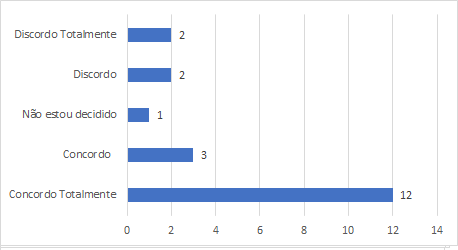
\includegraphics[scale=0.7]{figuras das questoes/2.13.png}
\caption{Respostas questão 2.13}

\paragraph{
Setenta e cinco por cento (75{\%}) dos respondentes se preocupam em resguardar a visualização da senha quando digitada.  Com esse resultado é possível  ver que existe uma preocupação dos desenvolvedores quanto a proteção da visualização da senha.
}
\label{fig:2.13}
\end{figure}


%aqui acaba uma figura
%--------------------------%
%aqui começa uma figura
\begin{figure}[!t]
\centering

\paragraph{Os respondentes foram questionados sobre a preocupação com o uso de criptografia para a proteção das informações sensíveis durante a comunicação em dispositivos móveis.  Os resultados podem ser consultados na figura \ref{fig:3.1}.
}
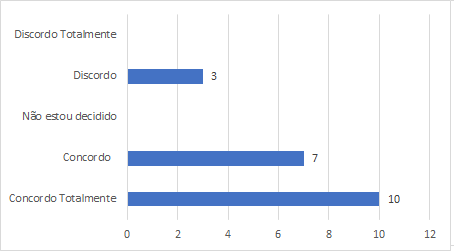
\includegraphics[scale=0.7]{figuras das questoes/3.1.png}
\caption{Respostas questão 3.1}

\paragraph{Oitenta e cinco por cento (85{\%}) dos participantes se preocupam usar criptografia para a proteção de informações, considerando tanto aqueles que concordam totalmente (50{\%}), quanto aqueles que apenas concordam (35{\%}). Com o resultado fica claro que existe uma preocupação dos desenvolvedores com a utilização de criptografia.
}

\label{fig:3.1}
\end{figure}
%aqui acaba uma figura
%--------------------------%
%aqui começa uma figura
\begin{figure}[!t]
\centering
\paragraph{
Os participantes foram questionados sobre a preocupação em gerar chaves para diferentes sistemas sistemas criptográficos e diferentes aplicações. s resultados podem ser consultados na figura \ref{fig:3.2}.}
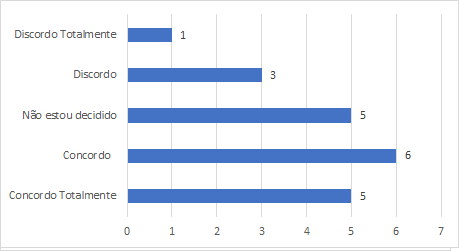
\includegraphics[scale=0.7]{figuras das questoes/3.2.png}
\caption{Respostas questão 3.2}

\paragraph{
Cinquenta e cinco por cento (55{\%}) dos participantes se preocupam em gerar chaves para diferentes sistemas criptográfico, 25{\%} não souberam opinar e 20{\%} discordam que seja uma preocupação. Com esse resultado é possível ver que a maioria dos desenvolvedores considera que gerar diferentes chaves criptográficas é importante.
}

\label{fig:3.2}
\end{figure}
%aqui acaba uma figura
%--------------------------%
%aqui começa uma figura
\begin{figure}[!t]
\centering

\paragraph{Os participantes foram questionados sobre a preocupação com os impactos da segurança da informação quando ocorre alguma mudança no sistema. Os resultados podem ser consultados na figura \ref{fig:4.1}.}
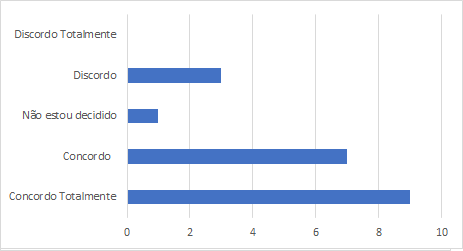
\includegraphics[scale=0.7]{figuras das questoes/4.1.png}
\caption{Respostas questão 4.1}
\paragraph{Oitenta por cento (85{\%}) do participantes se preocupam com os impactos da segurança da informação quando ocorre alguma mudança no sistema, considerando tanto aqueles que concordam totalmente (45{\%}), quanto aqueles que apenas concordam (35{\%}).Com esse resultado fica claro que existe uma preocupação dos desenvolvedores.}

\label{fig:4.1}
\end{figure}
%aqui acaba uma figura
%--------------------------%
%aqui começa uma figura
\begin{figure}[!t]
\centering
\paragraph{Os participantes foram questionados sobre a preocupação de  criar mecanismos para atender o crescimento da aplicação e possibilitar suportar demanda variável de acessos. Os resultados podem ser consultados na figura \ref{fig:4.2}.}

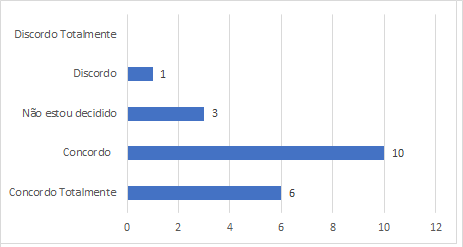
\includegraphics[scale=0.7]{figuras das questoes/4.2.png}
\caption{Respostas questão 4.2}
\paragraph{Oitenta por cento (80{\%}) dos participantes se preocupam em criar mecanismos para atender o crescimento da aplicação, considerando tanto aqueles que concordam totalmente (30{\%}), quanto aqueles que apenas concordam (50{\%}).Com esse resultado fica claro que existe uma preocupação dos desenvolvedores.}
\label{fig:4.2}
\end{figure}
%aqui acaba uma figura
%--------------------------%
%aqui começa uma figura
\begin{figure}[!t]
\centering
\paragraph{Os participantes foram questionados sobre a preocupação de não copiar dados sensíveis para o ambiente de teste. Os resultados podem ser consultados na figura \ref{fig:4.3}.}

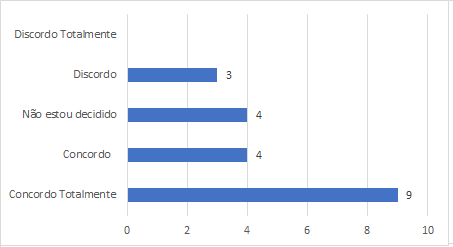
\includegraphics[scale=0.7]{figuras das questoes/4.3.png}
\caption{Respostas questão 4.3}
\paragraph{sessenta e cinco por cento (65{\%}) dos participantes se preocupam em não copiar dados sensíveis para o ambiante de teste, considerando tanto aqueles que concordam totalmente (45{\%}), quanto aqueles que apenas concordam (20{\%}).Com esse resultado fica claro que existe uma preocupação dos desenvolvedores em não copiar dados sensíveis para o ambiente de teste} 

\label{fig:4.3}
\end{figure}
%aqui acaba uma figura
%--------------------------%
%aqui começa uma figura
\begin{figure}[!t]
\centering
\paragraph{Os respondentes foram questionados sobre a preocupação em criarem mecanismos para registrar eventos no sistema. Os resultados podem ser consultados na figura \ref{fig:5.3.}}
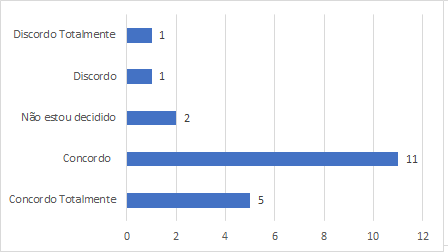
\includegraphics[scale=0.7]{figuras das questoes/5.1.png}
\caption{Respostas questão 5.1}
\paragraph{Oitenta por cento (85{\%}) dos participantes se preocupam em criar mecanismos para registrar eventos no sistema, considerando tanto aqueles que concordam totalmente (45{\%}), quanto aqueles que apenas concordam (20{\%}). Com esse resultado fica claro que existe uma preocupação dos desenvolvedores em registrar os eventos no sistema.}
\label{fig:5.1}
\end{figure}

%aqui acaba uma figura
%--------------------------%
%aqui começa uma figura

\begin{figure}[!t]
\centering
\paragraph{Os participantes foram questionados sobre a preocupação de registrar datas e horários de entrada e saída do sistema. Os resultados podem ser consultados na figura \ref{fig:5.3.}}
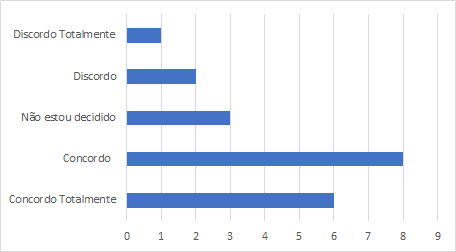
\includegraphics[scale=0.7]{figuras das questoes/5.2.png}
\caption{Respostas questão 5.2}
\paragraph{Setenta por cento (70{\%}) dos participantes se preocupam em registrar eventos de entrada e saída do sistema, considerando tanto aqueles que concordam totalmente (30{\%}), quanto aqueles que apenas concordam (40{\%}).Com esse resultado fica claro que existe uma preocupação dos desenvolvedores em registrar os eventos de datas e horários.}
\label{fig:5.3}
\end{figure}

%aqui acaba uma figura
%--------------------------%
%aqui começa uma figura

\begin{figure}[!t]
\centering
\paragraph{Os participantes foram questionados sobre a preocupação com a identificação do dispositivo ou sua localização quando possível. Os resultados podem ser consultados na figura \ref{fig:5.3}.}
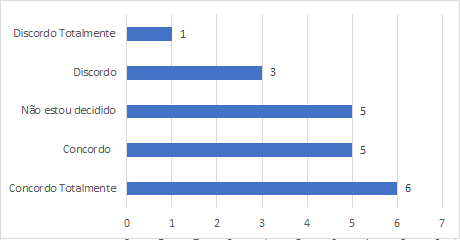
\includegraphics[scale=0.7]{figuras das questoes/5.3.png}
\caption{Respostas questão 5.3}
\paragraph{Cinquenta e cinco por cento (55{\%}) dos participantes se preocupam com localização ou identificação dos dispositivos, 25{\%} não soube opinar e 20{\%} discaram que seja uma preocupação. Com o resultado é possível ver que a maioria dos desenvolvedores se preocupa com a questão, entretanto uma parcela significativa não soube responder ou discordou.}
\label{fig:5.3}
\end{figure}

%aqui acaba uma figura
%--------------------------%
%aqui começa uma figura

\begin{figure}[!t]
\centering
\paragraph{Os participantes foram questionados sobre a preocupação de registrar tentativas de acesso ao sistema, sejam elas aceitadas ou rejeitadas. Os resultados podem ser consultados na figura \ref{fig:5.4}.}
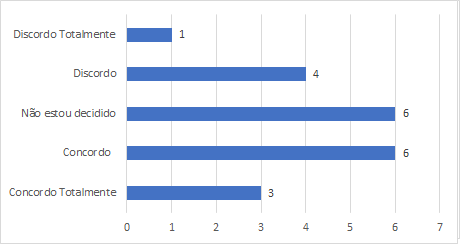
\includegraphics[scale=0.7]{figuras das questoes/5.4.png}
\caption{Respostas questão 5.4}
\paragraph{Quarenta e cinco por cento (45{\%}) dos participantes se preocupam em registrar tentativas de acesso ao sistema, 30{\%} não soube opinar e 25{\%} não acha que seja uma preocupação. Com o resultado não fica possível afirmar se existe uma preocupação dos desenvolvedores a respeito da questão.}
\label{fig:5.4}
\end{figure}
 %aqui acaba uma figura
%--------------------------%
%aqui começa uma figura
\begin{figure}[!t]
\centering
\paragraph{Os participantes foram questionados sobre a preocupação em coletar endereços e protocolos de rede no log. Os resultados podem ser consultados na figura \ref{fig:5.5}.}
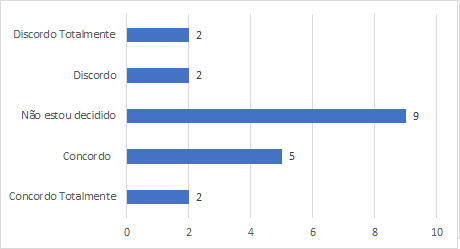
\includegraphics[scale=0.7]{figuras das questoes/5.5.png}
\caption{Respostas questão 5.5}
\paragraph{Trinta e cinco por cento (35{\%}) dos participantes se preocupam com a coleta de endereços e protocolos de rede, 45{\%} não soube opinar e 20{\%} não consideram como uma preocupação. Com o resultado não é possível afirmar se existe uma preocupação dos desenvolvedores, pois a maior parte dos respondentes não soube responder a questão.}
\label{fig:5.5}
\end{figure}
%aqui acaba uma figura
%--------------------------%
%aqui começa uma figura
\begin{figure}[!t]
\centering
\paragraph{Os respondentes foram questionados sobre a preocupação para que arquivos de log não sejam editados ou excluídos sem a devida autorização. Os resultados podem ser consultados na figura \ref{fig:5.6}.}
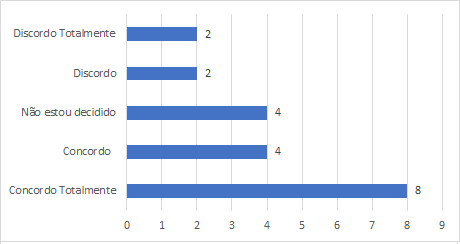
\includegraphics[scale=0.7]{figuras das questoes/5.6.png}
\caption{Respostas questão 5.6}
\paragraph{Sessenta por cento (60{\%}) dos participantes se preocupam com integridade dos arquivos de log,considerando tanto aqueles que concordam totalmente (40{\%}), quanto aqueles que apenas concordam (20{\%}). Com esse resultado é possível observar que existe uma preocupação dos desenvolvedores com a integridade dos logs. }
\label{fig:5.6}
\end{figure}
%aqui acaba uma figura
%--------------------------%
%aqui começa uma figura
\begin{figure}[!t]
\centering
\paragraph{Os respondentes foram questionados sobre a preocupação de identificar falhas de segurança nas aplicações que móveis que dão manutenção. Os resultados podem ser consultados na figura \ref{fig:6.1}.}
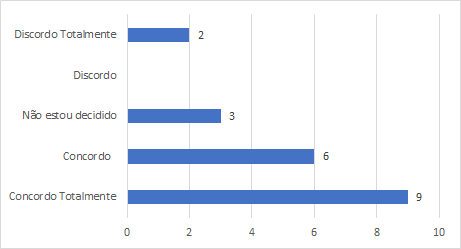
\includegraphics[scale=0.7]{figuras das questoes/6.1.png}
\caption{Respostas questão 6.1}
\paragraph{Setenta e cinco por cento (75{\%}) dos participantes se preocupam em identificar falhas de segurança, considerando tanto aqueles que concordam totalmente (40{\%}), quanto aqueles que apenas concordam (20{\%}). Com esse resultado é possível observar que existe uma preocupação dos desenvolvedores.
}
\label{fig:6.1}
\end{figure}
%aqui acaba uma figura
%--------------------------%
%aqui começa uma figura
\begin{figure}[!t]
\centering
\paragraph{Os respondentes foram questionados sobre a preocupação das informações envolvidas nos serviços de aplicação que transitam em redes que são de acesso público. Os resultados podem ser consultados na figura \ref{fig:6.2}.}
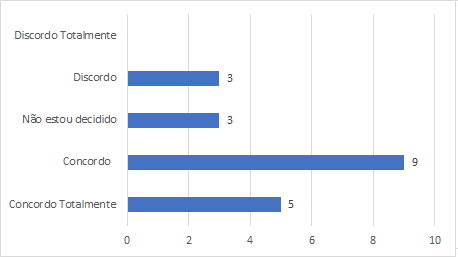
\includegraphics[scale=0.7]{figuras das questoes/6.2.png}
\caption{Respostas questão 6.2}
\paragraph{Setenta por cento (70{\%}) dos participantes se preocupam com as informações envolvidas nos serviços de aplicação em redes publicas, considerando tanto aqueles que concordam totalmente (25{\%}), quanto aqueles que apenas concordam (45{\%}). Com esse resultado é possível afirmar que a maior parte dos desenvolvedores se preocupam em proteger informações em redes públicas. }
\label{fig:6.2}
\end{figure}
%aqui acaba uma figura
%--------------------------%
%aqui começa uma figura
\begin{figure}[!t]
\centering
\paragraph{Os participantes foram questionados  sobre a preocupação em usar protocolos de comunicação seguros, para obter uma transação segura e confidencial. Os resultados podem ser consultados na figura \ref{fig:6.3}.}
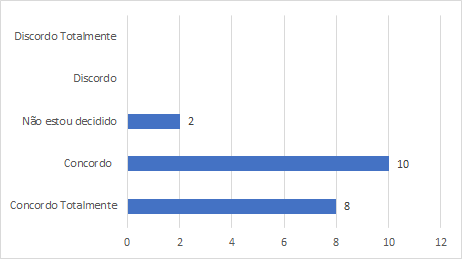
\includegraphics[scale=0.7]{figuras das questoes/6.3.png}
\caption{Respostas questão 6.3}
\paragraph{Noventa por cento (90{\%}) dos participantes se preocupam em usar protocolos de comunicação seguros para manter a confidencialidade. Com esse resultado fica claro que existe uma preocupação dos desenvolvedores mobile com a utilização de protocolos seguros.}
\label{fig:6.3}
\end{figure}
%aqui acaba uma figura
%--------------------------%
%aqui começa uma figura
\begin{figure}[!t]
\centering
\paragraph{ Os respondentes foram questionados sobre a preocupação em evitar que os detalhes de uma transação fiquem em um meio de armazenamento acessível diretamente pela internet, sem a devida segurança. Os resultados podem ser consultados na figura \ref{fig:6.4}.}
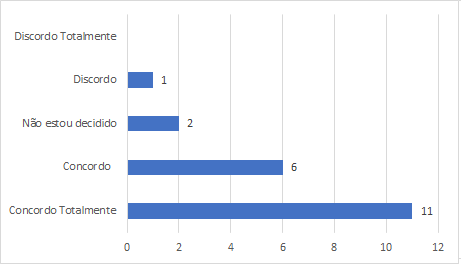
\includegraphics[scale=0.7]{figuras das questoes/6.4.png}
\caption{Respostas questão 6.4}
\paragraph{Oitenta e cinco por cento (85{\%}) dos participantes se preocupam em evitar que os detalhes de uma transação fiquem em uma armazenamento acessível diretamente pela internet. Com esse resultado fica claro que existe uma preocupação dos desenvolvedores mobile com o armazenamento de transações seguras. }
\label{fig:6.4}
\end{figure}
%aqui acaba uma figura
%--------------------------%
%aqui começa uma figura
\begin{figure}[!t]
\centering
\paragraph{Os participantes foram questionados sobre a preocupação em utilizar repositórios seguros para a construção de aplicações. Os resultados podem ser consultados na figura \ref{fig:6.5}}
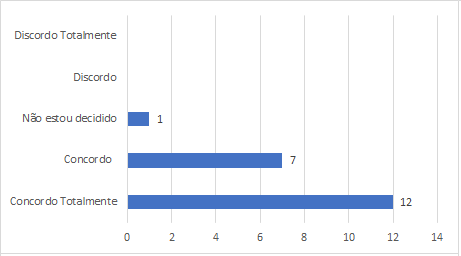
\includegraphics[scale=0.7]{figuras das questoes/6.5.png}
\caption{Respostas questão 6.5}
\paragraph{Noventa e cinco por cento (95{\%}) dos participantes se preocupam utilizar repositórios seguros. Com esse resultado fica claro que existe uma preocupação dos desenvolvedores mobile.}
\label{fig:6.5}
\end{figure}
%aqui acaba uma figura
%--------------------------%
%aqui começa uma figura
\begin{figure}[!t]
\centering
\paragraph{Os participantes foram questionados sobre a preocupação com a análise dos controles da aplicação e dos procedimentos de integridade para assegurar que eles não tenham sido comprometidos pelas mudanças na plataforma operacional. Os resultados podem ser consultados na figura \ref{fig:6.6}}
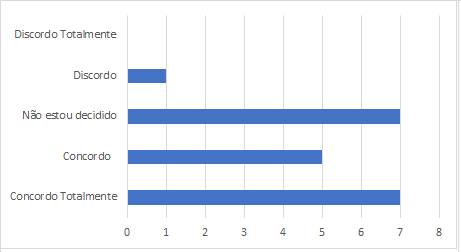
\includegraphics[scale=0.7]{figuras das questoes/6.6.png}
\caption{Respostas questão 6.6}
\paragraph{Sessenta por cento (60{\%}) dos participantes se preocupam, com a análise dos controles da aplicação, contudo {\%35} não soube responder.Com esse resultado é possível mostrar que existe uma preocupação dos desenvolvedores mobile, entretanto o número considerável de respostas neutras pode indicar que a questão não estivesse claro ou falta de entendimento.}
\label{fig:6.6}
\end{figure}
%aqui acaba uma figura
%--------------------------%
%aqui começa uma figura
\begin{figure}[!t]
\centering
\paragraph{Os participantes foram questionados sobre a preocupação de analisar novas tecnologias para serem aplicadas para reduzir os ricos de segurança. Os resultados podem ser consultados na figura \ref{fig:6.7}}
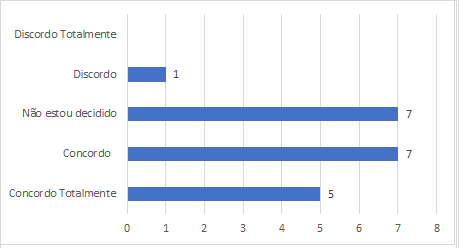
\includegraphics[scale=0.7]{figuras das questoes/6.7.png}
\caption{Respostas questão 6.7}
\paragraph{Sessenta por cento (60{\%}) dos participantes se preocupam em analisar novas tecnologias para redução de riscos de segurança e 35{\%} não soube opinar. Com esse resultado é possível afirmar que a maioria dos desenvolvedores se preocupa, entretanto o número considerável de respostas neutras pode indicar que a questão não estivesse claro ou falta de entendimento.}
\label{fig:6.7}
\end{figure}
%aqui acaba uma figura
%--------------------------%
%aqui começa uma figura
\begin{figure}[!t]
\centering
\paragraph{Os participante foram questionados sobre a preocupação em analisar riscos para prover o desenvolvimento da aplicação. Os resultados podem ser consultados na figura \ref{fig:6.8}}
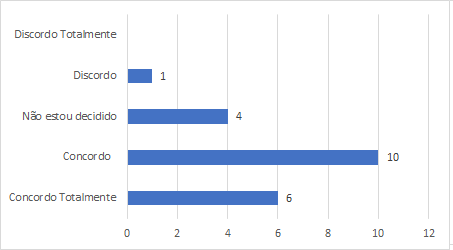
\includegraphics[scale=0.7]{figuras das questoes/6.8.png}
\caption{Respostas questão 6.8}
\paragraph{Oitenta por cento (80{\%}) do participantes se preocupam em analisar riscos de impacto para prover o desenvolvimento de segurança na aplicação, considerando tanto aqueles que concordam totalmente (30{\%}), quanto aqueles que apenas concordam (50{\%}). Com esse resultado fica claro que existe uma preocupação dos desenvolvedores mobile. }
\label{fig:6.8}
\end{figure}
%aqui acaba uma figura
%--------------------------%
%aqui começa uma figura
\begin{figure}[!t]
\centering
\paragraph{Os participantes foram questionados sobre a preocupação em separar diferentes ambientes de desenvolvimento. Os resultados podem ser consultados na figura \ref{fig:6.9}}
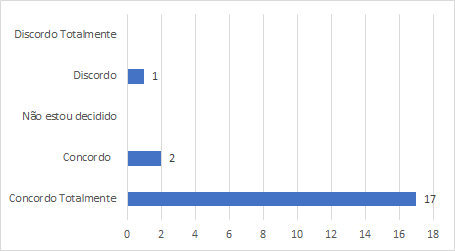
\includegraphics[scale=0.7]{figuras das questoes/6.9.png}
\caption{Respostas questão 6.9}
\paragraph{Noventa e cinco por cento (95{\%}) dos respondentes se preocupam em separar os ambientes de desenvolvimento,considerando tanto aqueles que concordam totalmente (85{\%}), quanto aqueles que apenas concordam (10{\%}).Com esse resultado fica evidente a preocupação dos desenvolvedores mobile com a separação dos ambientes. Com esse resultado fica claro que existe uma preocupação dos desenvolvedores mobile.}
\label{fig:6.9}
\end{figure}
%aqui acaba uma figura
%--------------------------%
%aqui começa uma figura
\begin{figure}[!t]
\centering
\paragraph{Os participantes foram questionados sobre a preocupação com a sensibilidade dos dados a serem processados, armazenados e transmitidos pelo sistema. Os resultados podem ser consultados na figura \ref{fig:6.10}}
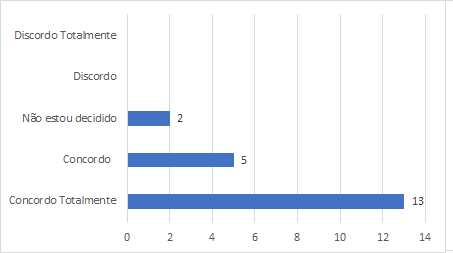
\includegraphics[scale=0.7]{figuras das questoes/6.10.png}
\caption{Respostas questão 6.10}
\paragraph{Noventa por cento (90{\%}) dos participantes se preocupam com a sensibilidade dos dados, considerando tanto aqueles que concordam totalmente (65{\%}), quanto aqueles que apenas concordam (25{\%}). Com esse resultado fica claro que existe uma preocupação dos desenvolvedores mobile.}
\label{fig:6.10}
\end{figure}
%aqui acaba uma figura
%--------------------------%
%aqui começa uma figura
\begin{figure}[!t]
\centering
\paragraph{Os participantes foram questionados sobre a preocupação em realizar testes de segurança em funcionalidades desenvolvidas. Os resultados podem ser consultados na figura \ref{fig:6.11}}
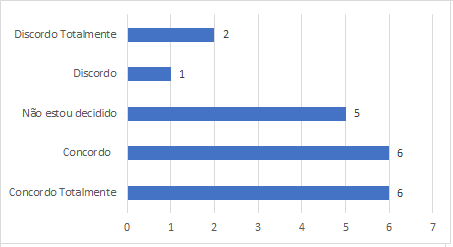
\includegraphics[scale=0.7]{figuras das questoes/6.11.png}
\caption{Respostas questão 6.11}
\paragraph{Sessenta por cento (60{\%}) dos participantes se preocupam em realizar testes de segurança em funcionalidades desenvolvidas, 25{\%} não soube responder e 15{\%} discordam que seja uma preocupação. Com esse resultado é possível ver que existe uma preocupação dos desenvolvedores em realizar testes de segurança.}
\label{fig:6.11}
\end{figure}
%aqui acaba uma figura
%--------------------------%
%aqui começa uma figura
\begin{figure}[!t]
\centering
\paragraph{Os respondentes foram questionados sobre a preocupação de realizar testes unitários. Os resultados podem ser consultados na figura \ref{fig:6.12}}
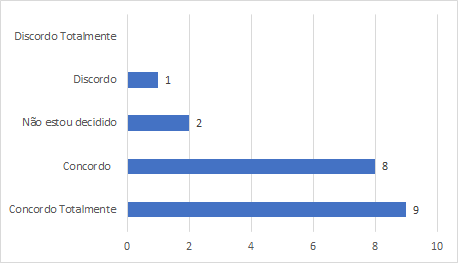
\includegraphics[scale=0.7]{figuras das questoes/6.12.png}
\caption{Respostas questão 6.12}
\paragraph{Oitenta e cinco por cento (85{\%}) dos respondentes se preocupam em realizar testes unitários, considerando tanto aqueles que concordam totalmente (45{\%}), quanto aqueles que apenas concordam (40{\%}). Com esse resultado fica claro que existe uma preocupação dos desenvolvedores mobile.}
\label{fig:6.12}
\end{figure}
%aqui acaba uma figura
%--------------------------%
%aqui começa uma figura
\begin{figure}[!t]
\centering
\paragraph{Os participantes foram questionados sobre a preocupação em realizar testes de funcionalidades desenvolvidas de maneira integrada no sistema. Os resultados podem ser consultados na figura \ref{fig:6.13}}
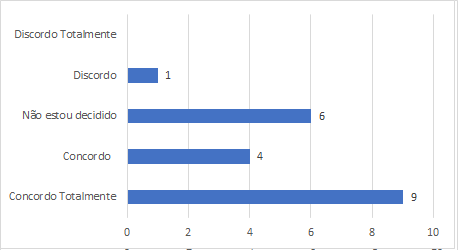
\includegraphics[scale=0.7]{figuras das questoes/6.13.png}
\caption{Respostas questão 6.13}
\paragraph{ Sessenta e cinco por cento (65{\%}) dos respondentes se preocupam em realizar testes de maneira integrada no sistema e 30{\%} não souber opinar. Com esse resultado é possível ver que existe uma preocupação dos desenvolvedores mobile, entretanto a quantidade de pessoal que não souberam opinar pode indicar que questão pudesse ser melhor elaborada}
\label{fig:6.13}
\end{figure}
%aqui acaba uma figura
%--------------------------%
%aqui começa uma figura
\begin{figure}[!t]
\centering
\paragraph{Os participantes foram questionados sobre a preocupação em utilizar ferramentes de análise de código. Os resultados podem ser consultados na figura \ref{fig:6.14}.}
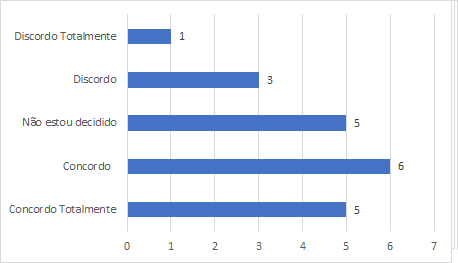
\includegraphics[scale=0.7]{figuras das questoes/6.14.png}
\caption{Respostas questão 6.14}
\paragraph{Cinquenta e cinco por cento (55{\%}) dos participantes se preocupam em utilizar ferramentas de análise de código, 25{\%} não soube responder e 20{\%} discordam que seja uma preocupação. Com o resultado é possível ver que a maioria dos desenvolvedores se preocupa, entretanto uma quantidade considerável não soube opinar ou discordou.}
\label{fig:6.14}
\end{figure}
%aqui acaba uma figura
%--------------------------%
%aqui começa uma figura
\begin{figure}[!t]
\centering
\paragraph{Os participantes foram questionados sobre a preocupação em realizar testes de aceitação no sistema. Os resultados podem ser consultados na figura \ref{fig:6.15}}
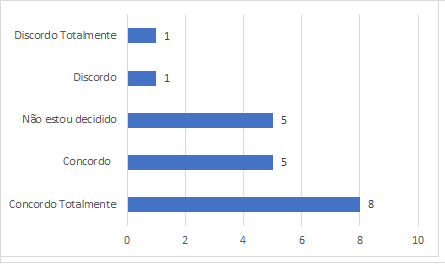
\includegraphics[scale=0.7]{figuras das questoes/6.15.png}
\caption{Respostas questão 6.15}
\paragraph{Sessenta e cinco por cento (65{\%}) dos entrevistados se preocupam em realizar testes de aceitação, 25{\%} não soube responder e 10{\%} discordou que que fosse uma preocupação. Com o resultado é possível ver a maioria dos desenvolvedores se preocupa com a realização de testes de aceitação.}
\label{fig:6.15}
\end{figure}
%aqui acaba uma figura
%--------------------------%
%aqui começa uma figura
\begin{figure}[!t]
\centering
\paragraph{Os participantes foram questionados sobre a preocupação com os dados de testes, caso o banco operacional seja utilizado. Os resultados podem ser consultados na figura \ref{fig:6.16}}
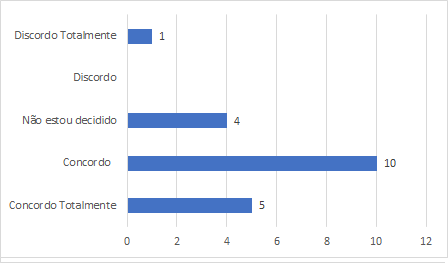
\includegraphics[scale=0.7]{figuras das questoes/6.16.png}
\caption{Respostas questão 6.16}
\paragraph{Setenta e cinco por cento (75{\%}) dos participam se preocupam com proteção dos dados de teste, caso o banco operacional seja utilizado, ,considerando tanto aqueles que concordam totalmente (25{\%}), quanto aqueles que apenas concordam (50{\%}).  Com esse resultado é possível ver que existe uma preocupação dos desenvolvedores.}
\label{fig:6.16}
\end{figure}
%aqui acaba uma figura
%--------------------------%
%aqui começa uma figura
\begin{figure}[t]
\centering
\paragraph{Os participantes foram questionados sobre a preocupação em proteger os dados do banco de dados operacional contra remoção e modificação. Os resultados podem ser consultados na figura \ref{fig:6.17}}
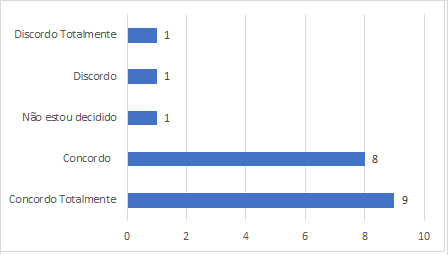
\includegraphics[scale=0.7]{figuras das questoes/6.17.png}
\caption{Respostas questão 6.17}
\paragraph{Oitenta e cinco por cento (85{\%}) dos participantes se preocupam em proteger os dados do banco operacional. Com esse resultado é possível ver que existe uma preocupação dos desenvolvedores.}
\label{fig:6.17}
\end{figure}




 

 

 
